\chapter{Experimental Simulation}  

The proposed \gls{bfast} algorithm will be tested using an experimental framework 
mimicking a single-subject \gls{fmri} experiment. The datasets from this 
experiments consist of the measured \gls{bold} signal for each voxel throughout 
the experiment. Also, it contains a structured log of the events during the experiment, 
which includes, among other things, stimulus times and duration. 

\section{Generation of the Simulated Framework}

The first step to creating a simulated framework is to identify true maps of the 
activated regions that will be distorted for the simulation. The \gls{bfast} algorithm 
will then be used to reconstruct the activation maps, and the results will be compared to 
the original true maps to measure the algorithm's accuracy. In this true maps, each voxel 
will be assigned a value of 0 if it is not activated and 1 if it is activated. To address 
different spatial structures, \gls{2d} and \gls{3d} true maps are considered. 
See Table \ref{tab:aMaps} for more details on the true maps.

\begin{table}[htbp!]
\centering
\caption{Details of True Maps Considered: In both maps, dark voxels are active and 
light voxels are inactive.}
\begin{tabular}{x{2.1cm}x{6cm}x{6cm}}
\hline
\textbf{Name} & \textbf{\gls{2d}} & \textbf{\gls{3d}} \\ \hline
Dimensions & $200 \times 200$ & $40 \times 40 \times 25$ \\
Voxels & 40000 & 40000 \\ 
\acrshort{poa} & 19.9375 & 3.9525 \\
Map & 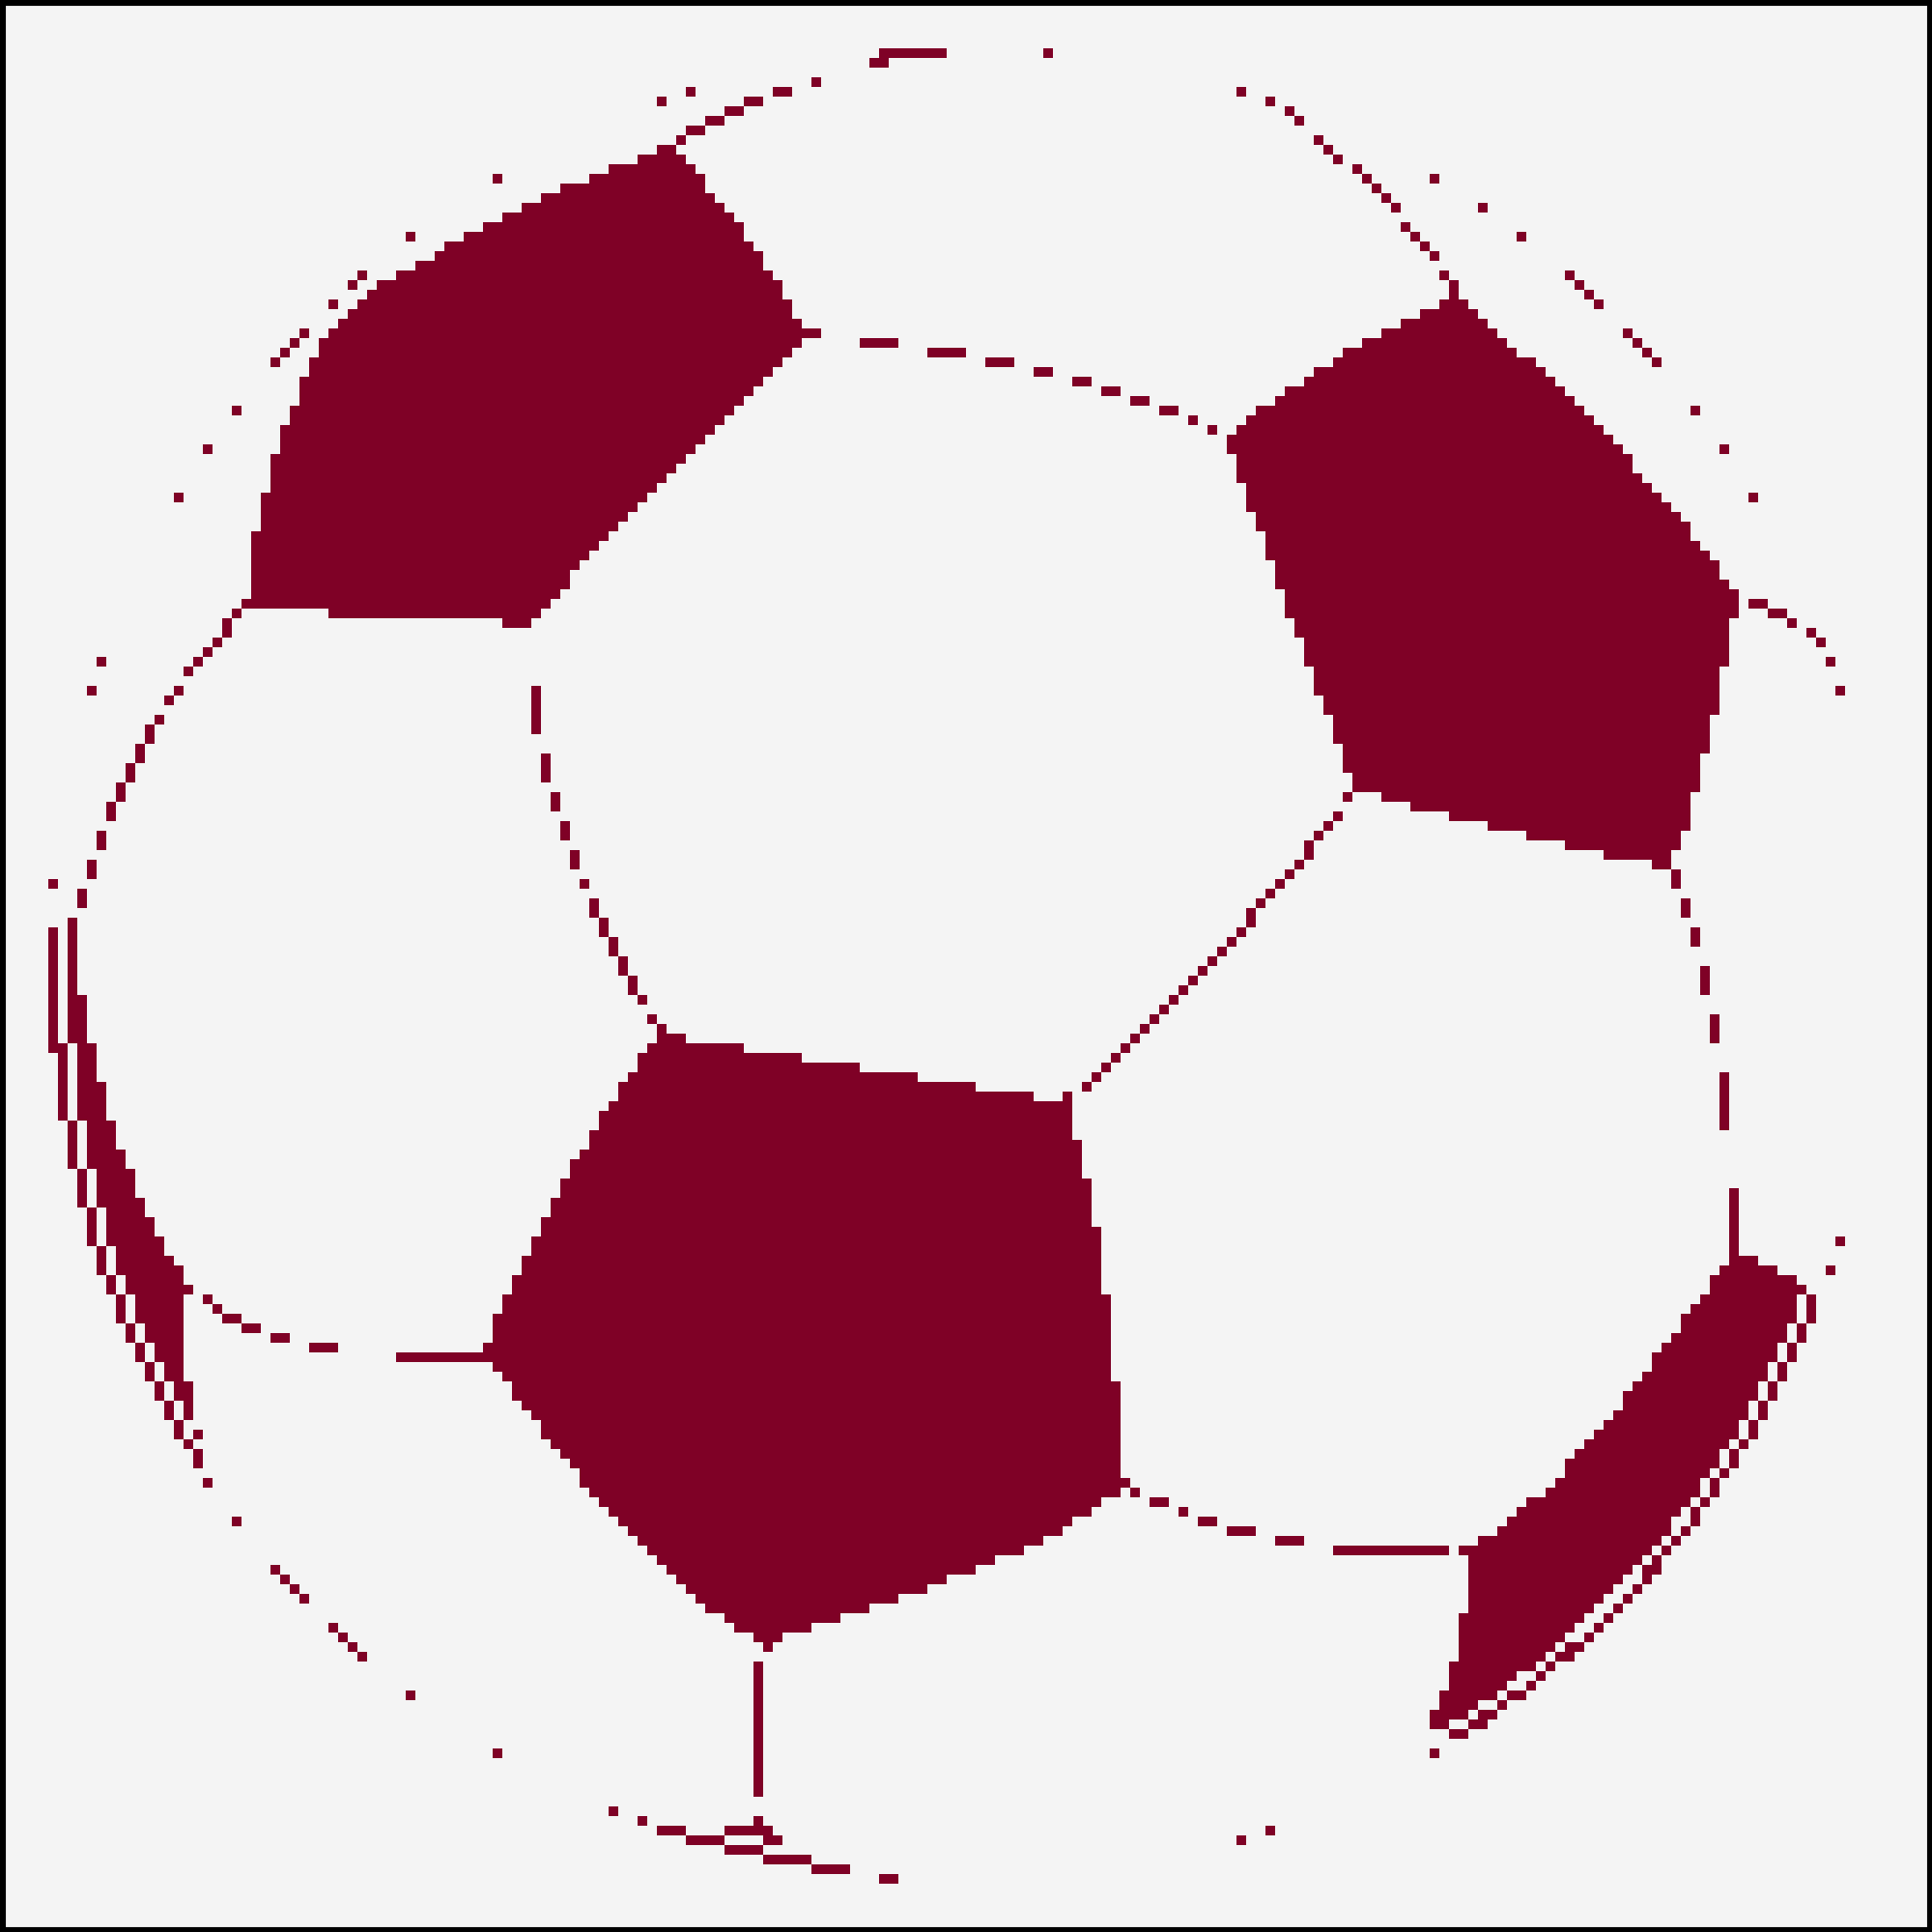
\includegraphics[width=0.35\textwidth]{images/aMap2D.png} & 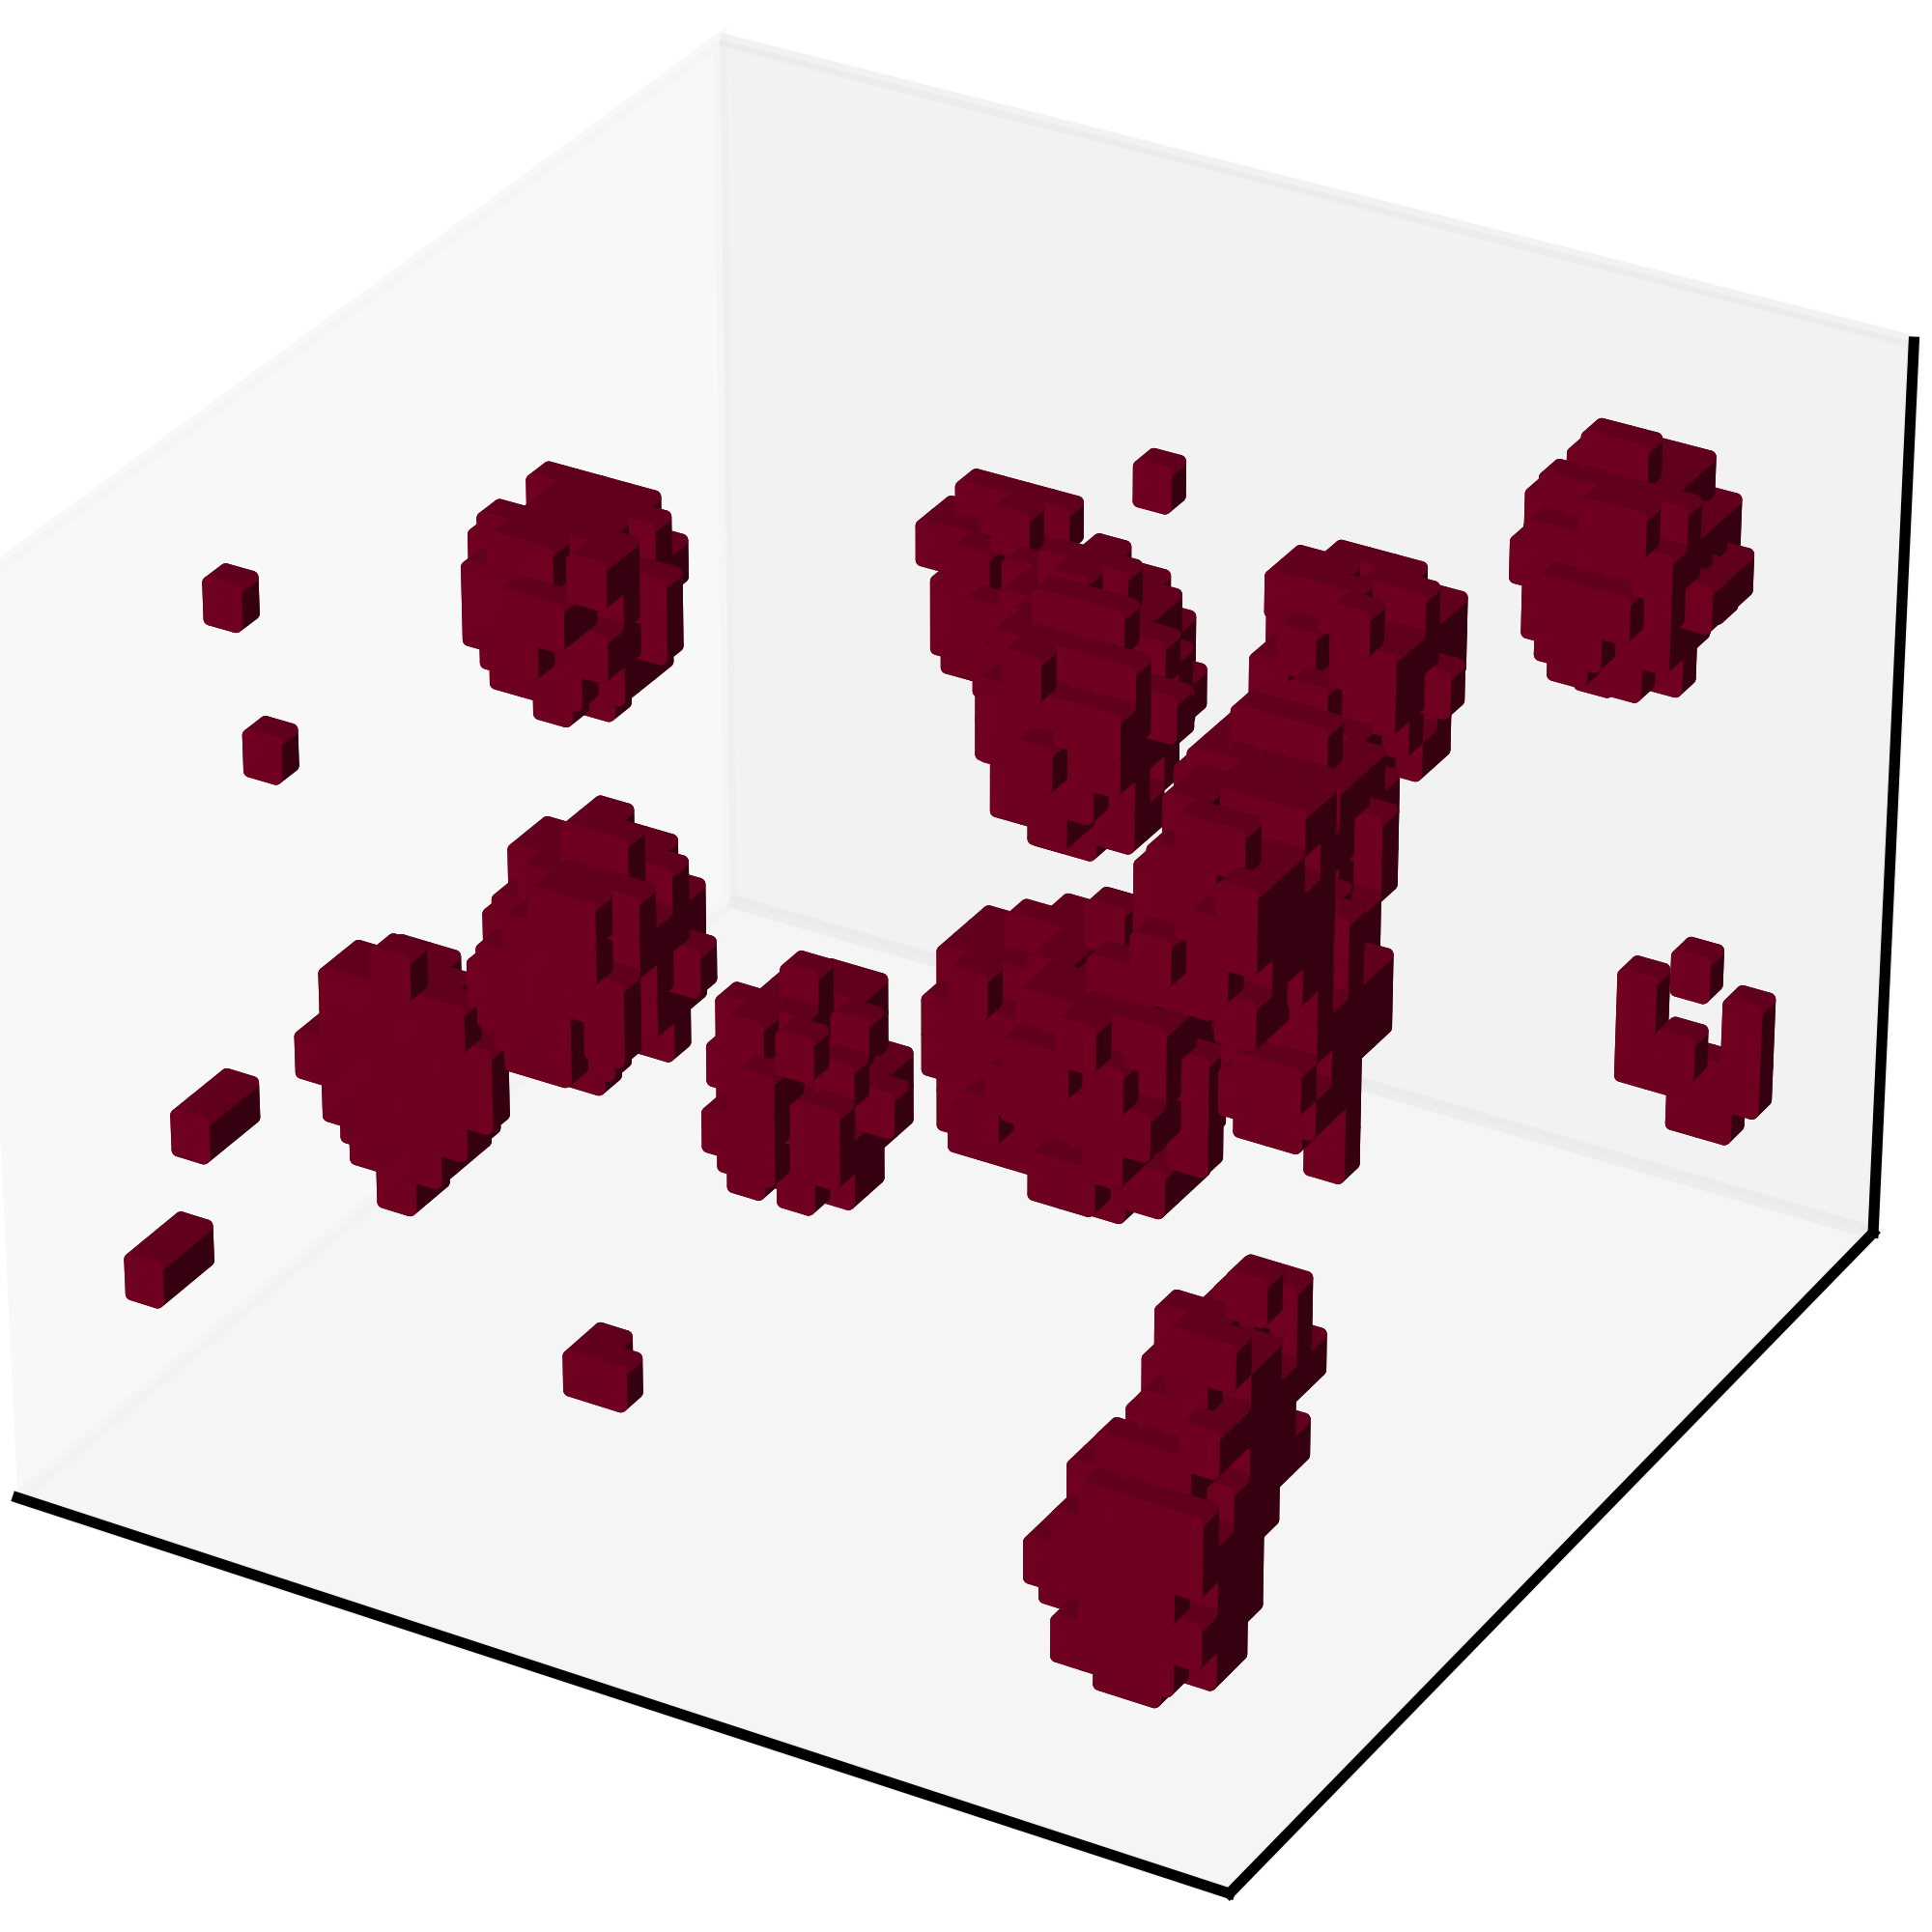
\includegraphics[width=0.35\textwidth]{images/aMap3D.png} \\ 
Source & Derived from File in Open Clip Art Library (Public Domain) & See Appendix \ref{ap:3dMapsGen} \\ \hline
\end{tabular}
\label{tab:aMaps}
\end{table}

The next step of the framework-building process is the creation of a design matrix of 
two columns, $\bm{X}$. The second column corresponds to the constant regressor and the 
first column contains the Glover \gls{hrf} \cite{lu2006using}, given specific event 
descriptions of an \gls{fmri} experiment. For the simulated framework, a single type 
of stimulus will be considered as the event of the \gls{fmri} experiment, however, this 
event will occur at different times. See Table \ref{tab:eventsSim} for the parameters 
chosen in this simulation.

\begin{table}[htbp!]
\centering
\caption{Event Description of Simulated \gls{fmri} Experiment.}
\begin{tabular}{lc}
\hline
\textbf{Parameter} & \textbf{Value} \\ \hline
Number of Scans & 100 \\
Time Between Scans & 2 seconds \\
Number of Stimulus & 4 \\
Duration of Each Stimulus & 10 seconds \\
Time Between Stimulus & 18 - 25 seconds \\ \hline
\end{tabular}
\label{tab:eventsSim}
\end{table}

Resulting then in the \gls{hrf} shown in Figure \ref{fig:gloverHRF}.

\begin{figure}[htbp!]
\centering
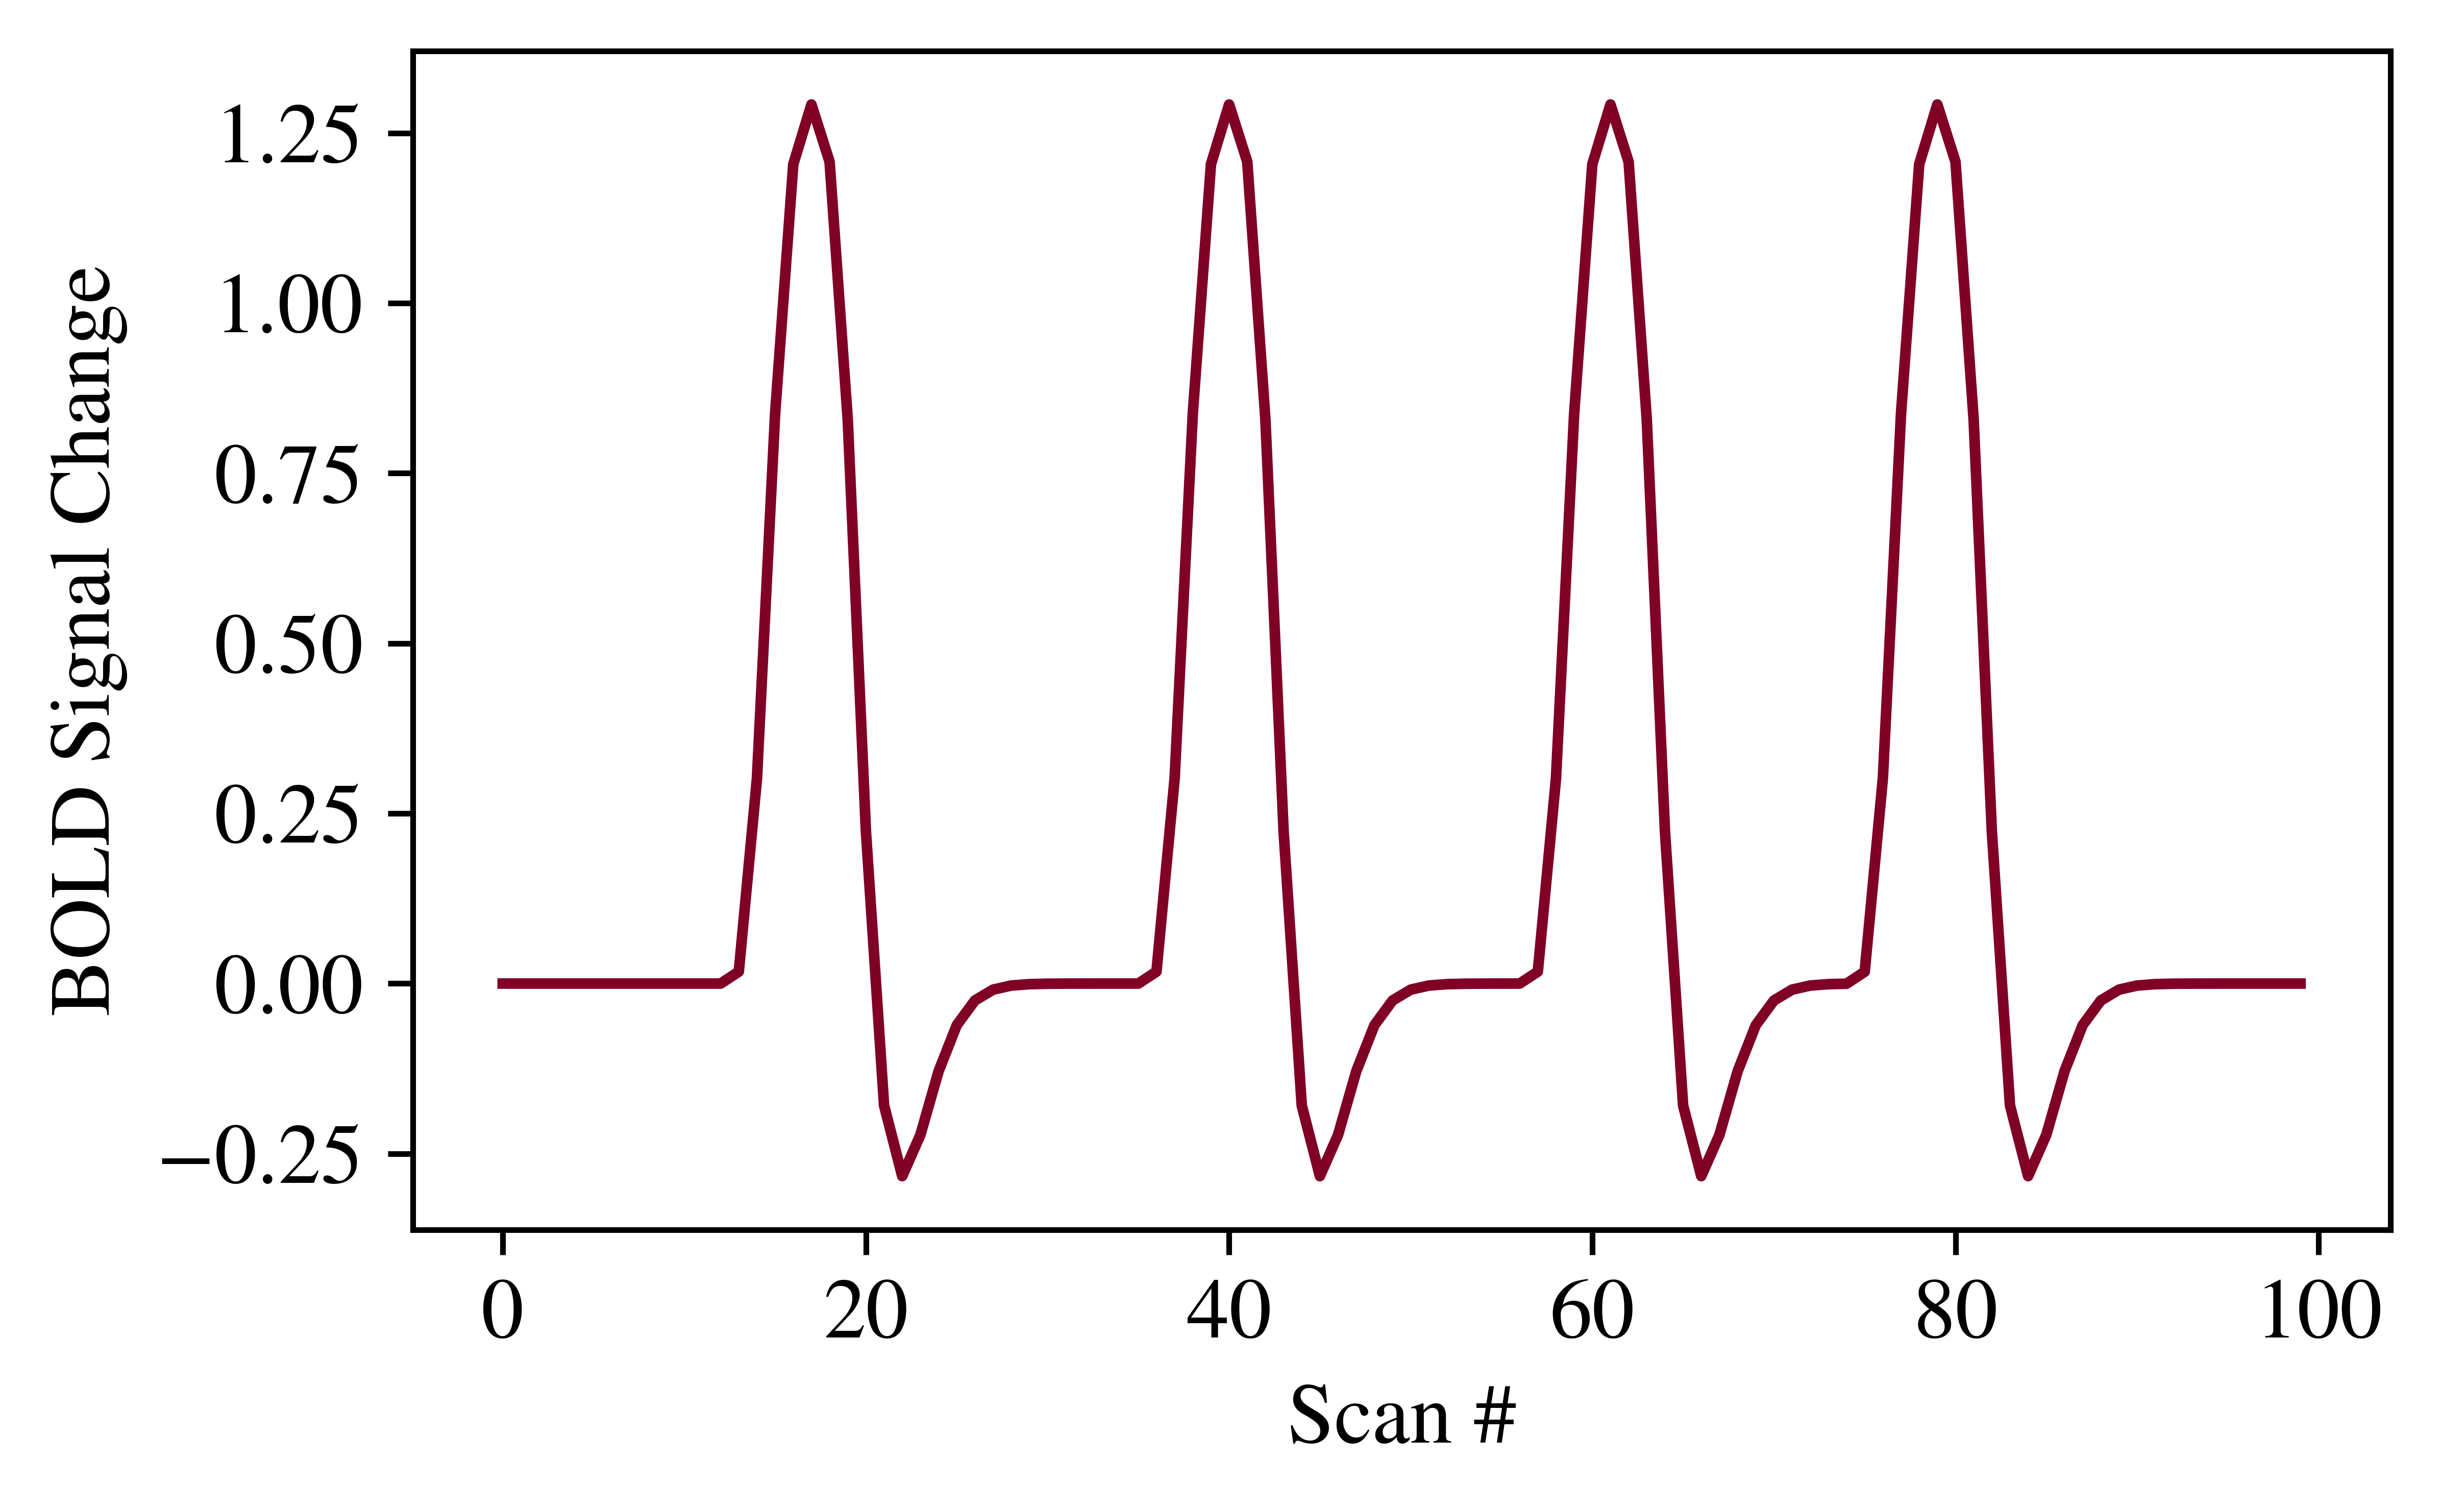
\includegraphics{images/gloverHRF.png}
\caption{Glover \gls{hrf} Given a Stimulus Described by Table \ref{tab:eventsSim}.}
\label{fig:gloverHRF}
\end{figure}

The final step in building the simulated framework is to compute the \gls{bold} response
, $\bm{y}_i$, for each voxel $i$. This process is divided into two steps: first, the 
computation of the \gls{bold} response without noise, and then, using an $ARMA$ Model 
to generate noise in the signal \cite{choi2012arma}, i.e.:
$
\bm{y}_i = \bm{X}\bm{\beta^*}_i + \bm{\epsilon}.
$

To compute the \gls{bold} response without noise we will set values for the parameter 
$\bm{\beta^*}_i$ depending on the voxel activation status, $\zeta_i$, on the true map as 
shown in Table \ref{tab:betaParameter}. The response is then computed as seen in 
Equation \ref{eq:boldCleanCalc}.

\begin{table}[htbp!]
\centering
\caption{Parameter Selection Based on Activation Status}
\begin{tabular}{cc}
\hline
\textbf{Activation Status} & \textbf{Parameter Values} \\ \hline
$\zeta_i=0$ & $\bm{\beta^*}_i = (0,100)^T$ \\
$\zeta_i=1$ & $\bm{\beta^*}_i = (75,100)^T$ \\ \hline
\end{tabular}
\label{tab:betaParameter}
\end{table}

\begin{equation} \label{eq:boldCleanCalc}
\bm{y^*}_i = \bm{X}\bm{\beta^*}_i
\end{equation}

On the other side, the noise ($\bm{\epsilon}$) is a vector of mean $\mu_{ARMA} = 0$ and 
variance $\sigma_{ARMA}^2=25^2$ with a baseline structure equivalent to 
${ARMA}_{\bm{\epsilon}}\left( \{p_1,p_2,\dots\},\{q_1,q_2,\dots\} \right)$. 
Note that $p = \left| \{p_1,p_2,\dots\} \right|$ and $q= \left| \{q_1,q_2,\dots\} \right|$ 
are related to the order of the corresponding $ARMA$ model. Also, $p_a$ and $q_b$ represent 
the coefficients of such models. Values of $p,q \in [0,1,2,3]$ were chosen to 
study the model under different noise scenarios. The values of $p_a$, 
and $q_b$ were chosen arbitrarily as parameters, see Table \ref{tab:noiseParameters}. Given the
values chosen for $\bm{\beta^*}_i$ when voxels are active and the value chosen for $\sigma_{ARMA}$,
the simulations are expected to have approximate \gls{snr} and \gls{cnr} values of 4 and 3, respectively.
Additionally, given the $ARMA$ structure of $\bm{\epsilon}$, the simulations with higher values of $p$ and
$q$ are expected to present bigger diffculties when detecting activation.

\begin{table}[htbp!]
\centering
\caption{Parameter Selection Related to $\bm{\epsilon}$}
\begin{tabular}{cccccc}
&&\multicolumn{4}{c}{$p$} \\
&\hspace{6pt} \arrvline&0&1&2&3 \\ \cline{2-6}
\multirow{4}{*}{$q$}&0 \arrvline & $\{\},\{\}$&$\{\frac{1}{2}\},\{\}$&$\{\frac{1}{2},\frac{3}{10}\},\{\}$&$\{\frac{1}{2},\frac{3}{10},\frac{1}{10}\},\{\}$ \\
&1 \arrvline & $\{\},\{\frac{1}{2}\}$&$\{\frac{1}{2}\},\{\frac{1}{2}\}$&$\{\frac{1}{2},\frac{3}{10}\},\{\frac{1}{2}\}$&$\{\frac{1}{2},\frac{3}{10},\frac{1}{10}\},\{\frac{1}{2}\}$ \\
&2 \arrvline & $\{\},\{\frac{1}{2},\frac{3}{10}\}$&$\{\frac{1}{2}\},\{\frac{1}{2},\frac{3}{10}\}$&$\{\frac{1}{2},\frac{3}{10}\},\{\frac{1}{2},\frac{3}{10}\}$&$\{\frac{1}{2},\frac{3}{10},\frac{1}{10}\},\{\frac{1}{2},\frac{3}{10}\}$ \\
&3 \arrvline & $\{\},\{\frac{1}{2},\frac{3}{10},\frac{1}{10}\}$&$\{\frac{1}{2}\},\{\frac{1}{2},\frac{3}{10},\frac{1}{10}\}$&$\{\frac{1}{2},\frac{3}{10}\},\{\frac{1}{2},\frac{3}{10},\frac{1}{10}\}$&$\{\frac{1}{2},\frac{3}{10},\frac{1}{10}\},\{\frac{1}{2},\frac{3}{10},\frac{1}{10}\}$
\end{tabular}
\label{tab:noiseParameters}
\end{table}